\chapter{Results of the measurements and interpretations}
\label{Chap4}

In this part, I will present the results of the mesurements I have made, both room temperature and low temperature measurements, and I will get the informations that we can get from these results.

\section{Room Temperature Results}
                \subsection{Reference Samples}
                
                Before starting to use the Plasma, I need to have some references to compare to the results with Plasma. I have made several references samples : a clean contact, a strong oxidation and a regular oxidation.
                
                I first made a clean contact sample, with only Al and Cu as a reference (See Fig.\ref{SEMcleancontact}). Since the contact is clean, the resistance of the junction between the two metals is close to zero, then the resistance we measure belongs to the leads which are following the following law :
                \[R=\sum_{Al,Cu}\dfrac{\rho L}{S}\]
                
                Since all the leads are the same, the resistance does not depends on the surface area of the junction, as you can see in Fig. \ref{cleancontact} the results of four probes measurements.
                The theoretical calculus from this law with the parameters used gives $78\Omega$, which is close to the value we find. Of course, there are some uncertainties : the thickness sensor in the evaporator is not very accurate, since we evaporate with an angle, the dimension are a bit different on the actual junctions, from the pattern dimension. The point is that the order of magnitude is correct, so our reference for the leads resistance will be around $70\Omega$.
                \begin{figure}
                    \centering
                    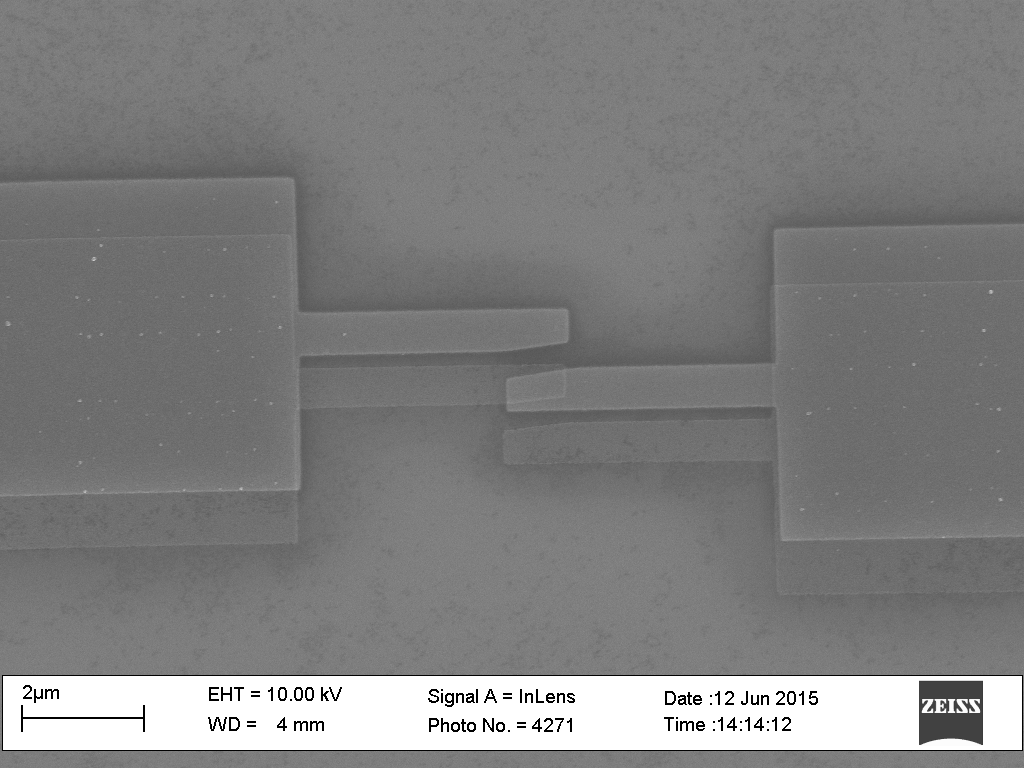
\includegraphics[width=6cm]{SEMtest12_1.png}
                    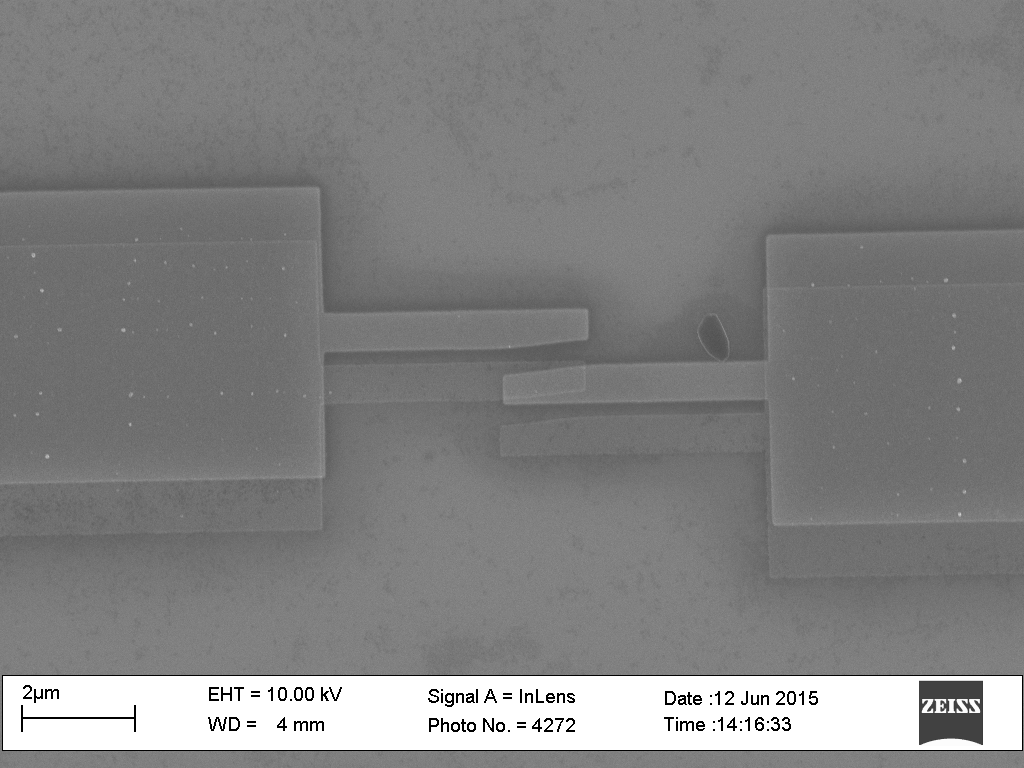
\includegraphics[width=6cm]{SEMtest12_2.png}
                    \caption{SEM images of the clean contact samples}
                    \label{SEMcleancontact}
                \end{figure}
                
                \begin{figure}
                    \centering
                    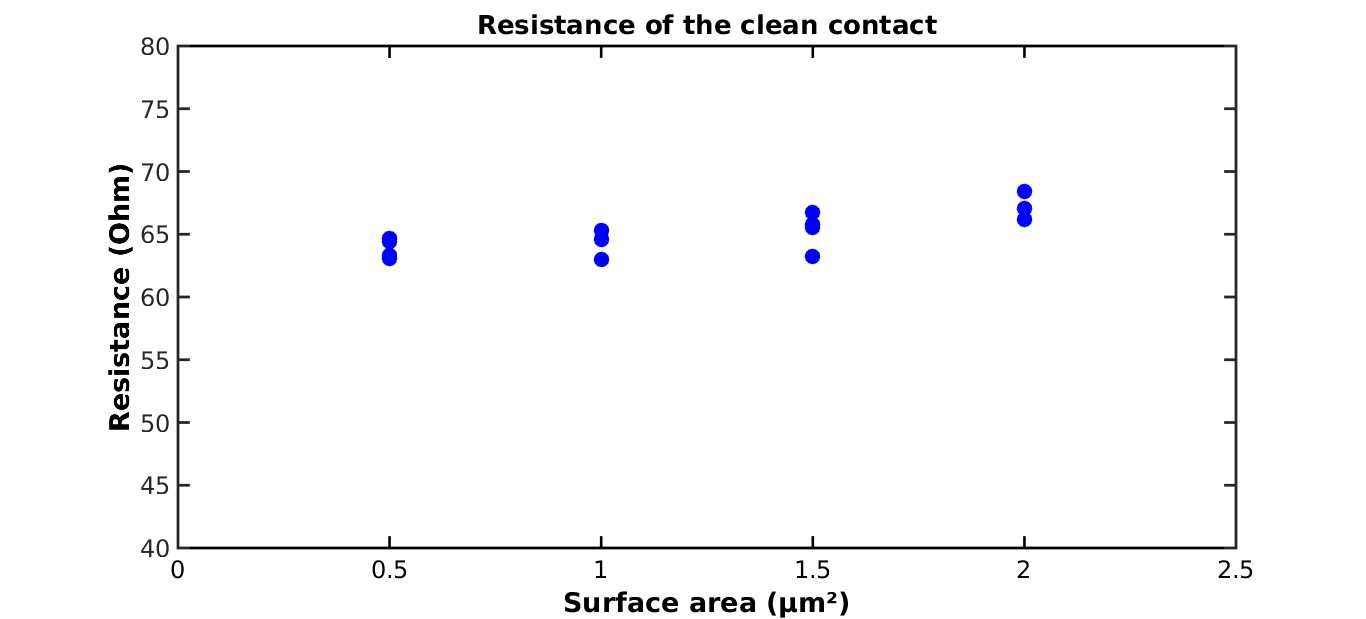
\includegraphics[width=12cm]{Rclean.png}
                    \caption{Resistance of clean contact in function of the surface area}
                    \label{cleancontact}
                \end{figure}
                
           
                After the clean contact, I made some reference samples for a strong oxidation, I oxidized freshly evaporated Al under a pressure of 200mbar during 10 minutes before evaporating Cu. The SEM images can be seen on Figure \ref{SEMstrongox}.
                
                \begin{figure}
                    \centering
                    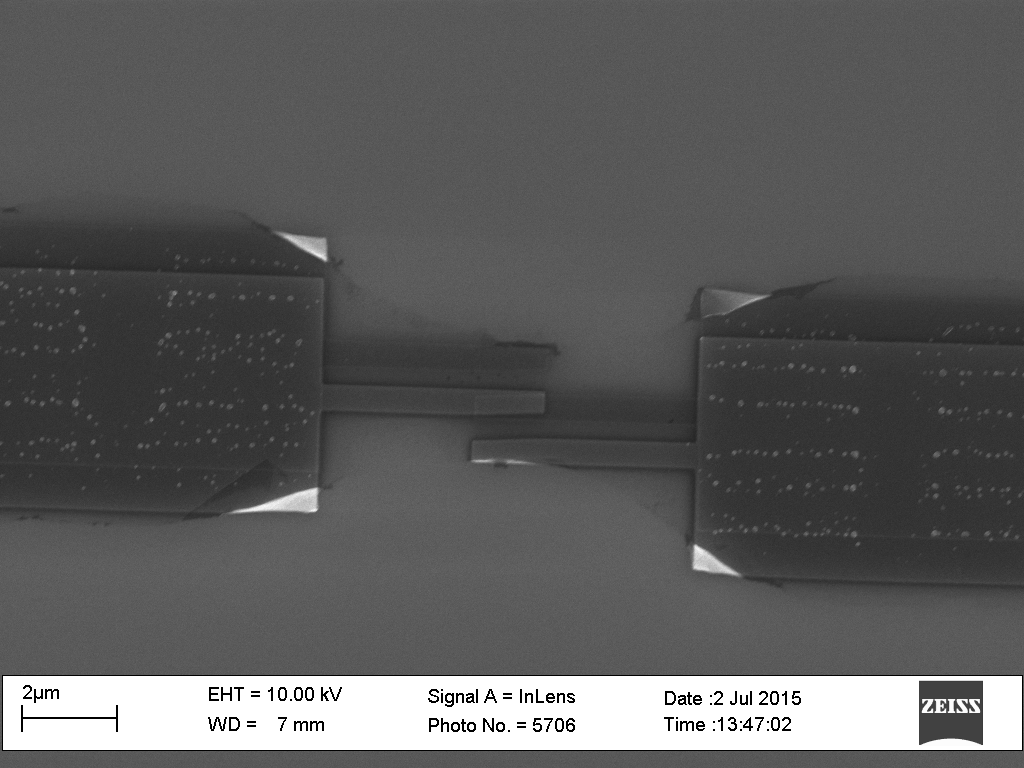
\includegraphics[width=6cm]{SEMtest15_1.png}
                    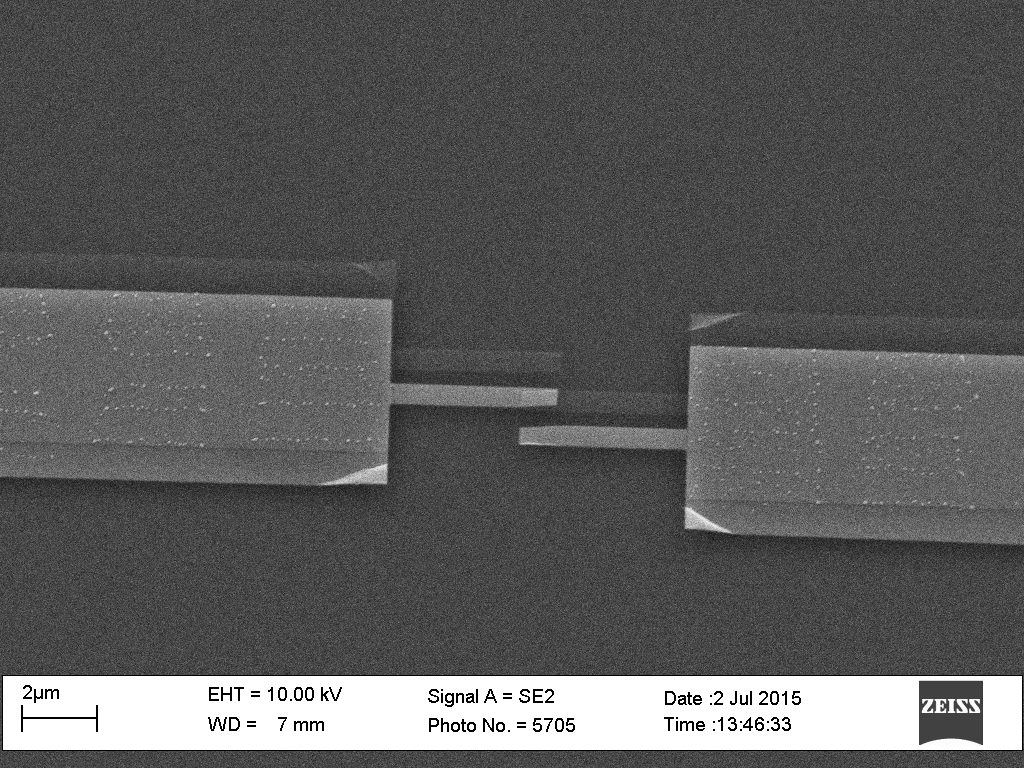
\includegraphics[width=6cm]{SEMtest15_2.png}
                    \caption{SEM images of the Strong Oxidation samples}
                    \label{SEMstrongox}
                \end{figure}
                
                For the NIS junctions, it is more relevant to draw conductance in function of the surface area of the junction so that we obtain a linear curve (See Fig. \ref{Strongox}), and we can determine the RS factor.
                
                \[RS=7.18k\Omega.\mu m^2\]
                
                This factor is relevant because : 
                \[R=\dfrac{\rho l}{S}\,\Longrightarrow\,l=\dfrac{RS}{\rho}\]
                
                In the case of the oxide, l is the thickness of the oxide layer, so that RS is proportional to the thickness.   
                
                \begin{figure}
                    \centering
                    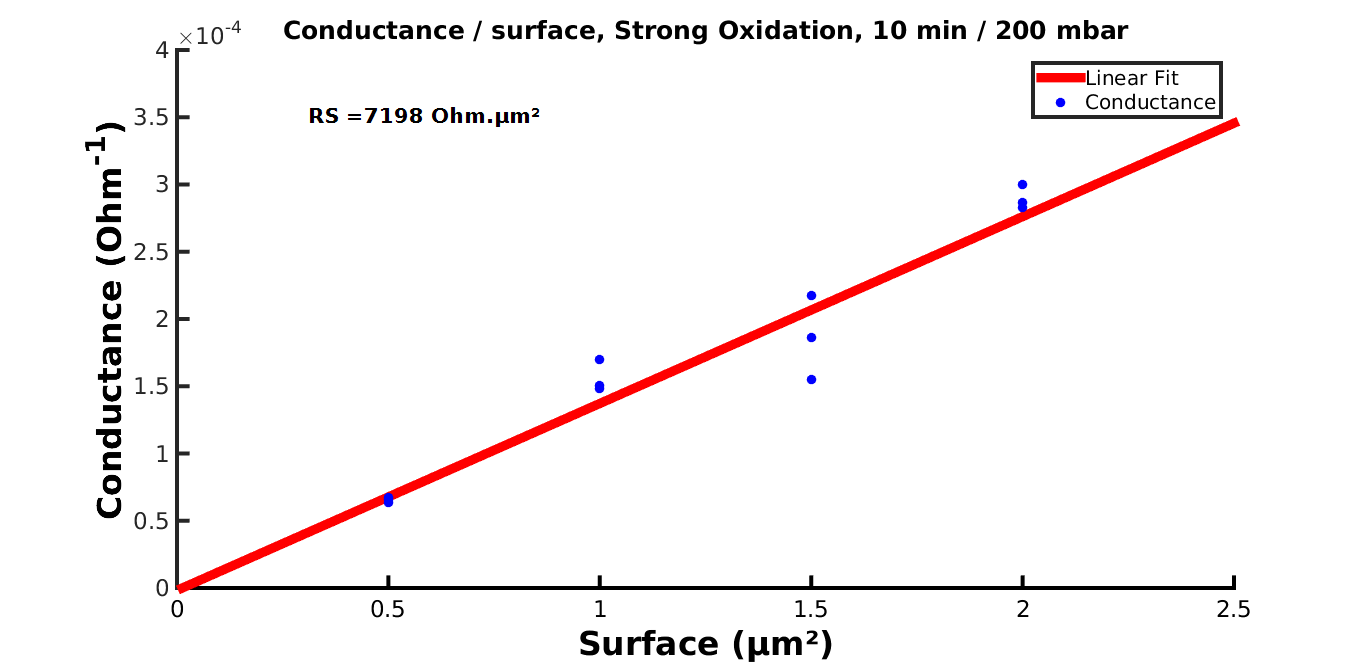
\includegraphics[width=12cm]{ConductanceFitStrongOx.png}
                    \caption{Conductance in function of surface area for a strong oxidized sample}
                    \label{Strongox}
                \end{figure}
                
                In order to cover a large range of resistance, I have also made a regular oxidation reference sample, with the evaporation of Al placed under 2mbar for 2 minutes before evaporating Cu.
                
                 \begin{figure}
                    \centering
                    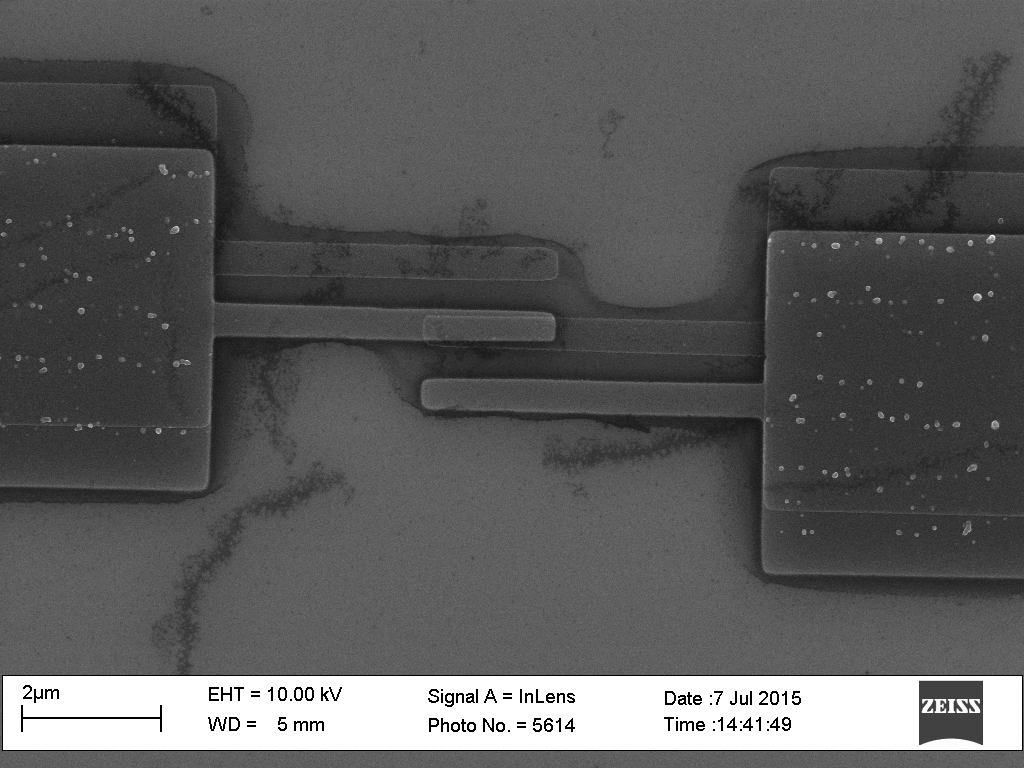
\includegraphics[width=6cm]{SEMtest16_1.png}
                    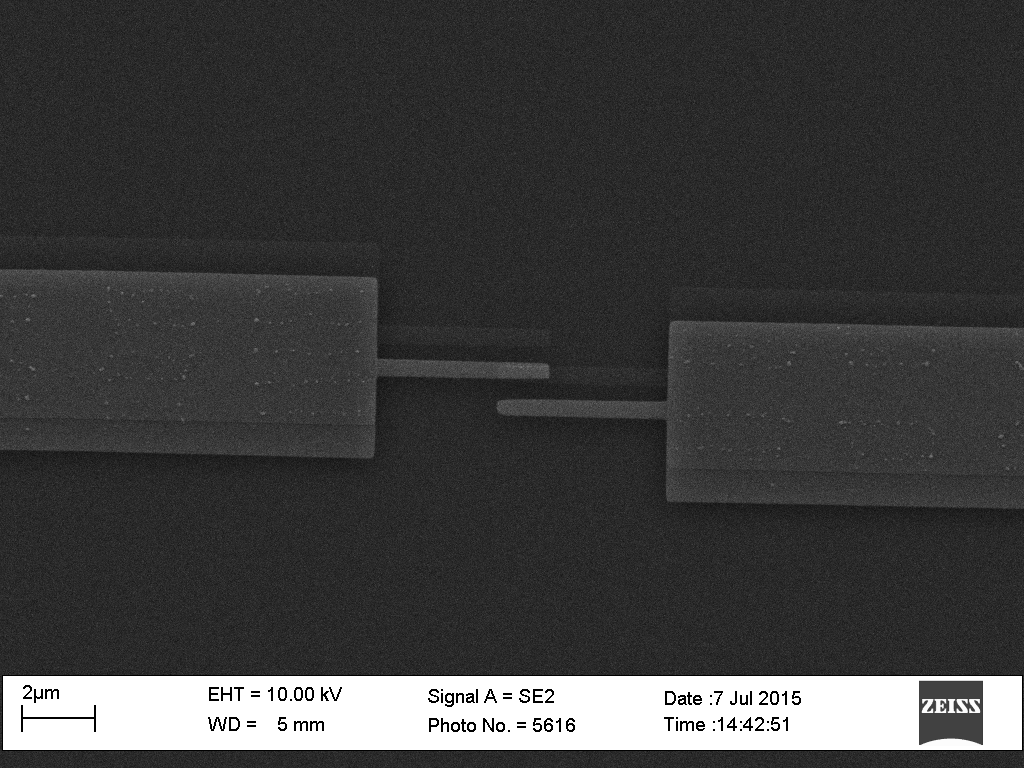
\includegraphics[width=6cm]{SEMtest16_2.png}
                    \caption{SEM images of the Regular Oxidation samples}
                    \label{SEMregularox}
                \end{figure}
                
                Again, it is more relevant to draw the conductance (See Fig. \ref{Regularox}) to determine the RS factor.
                
                \begin{figure}
                    \centering
                    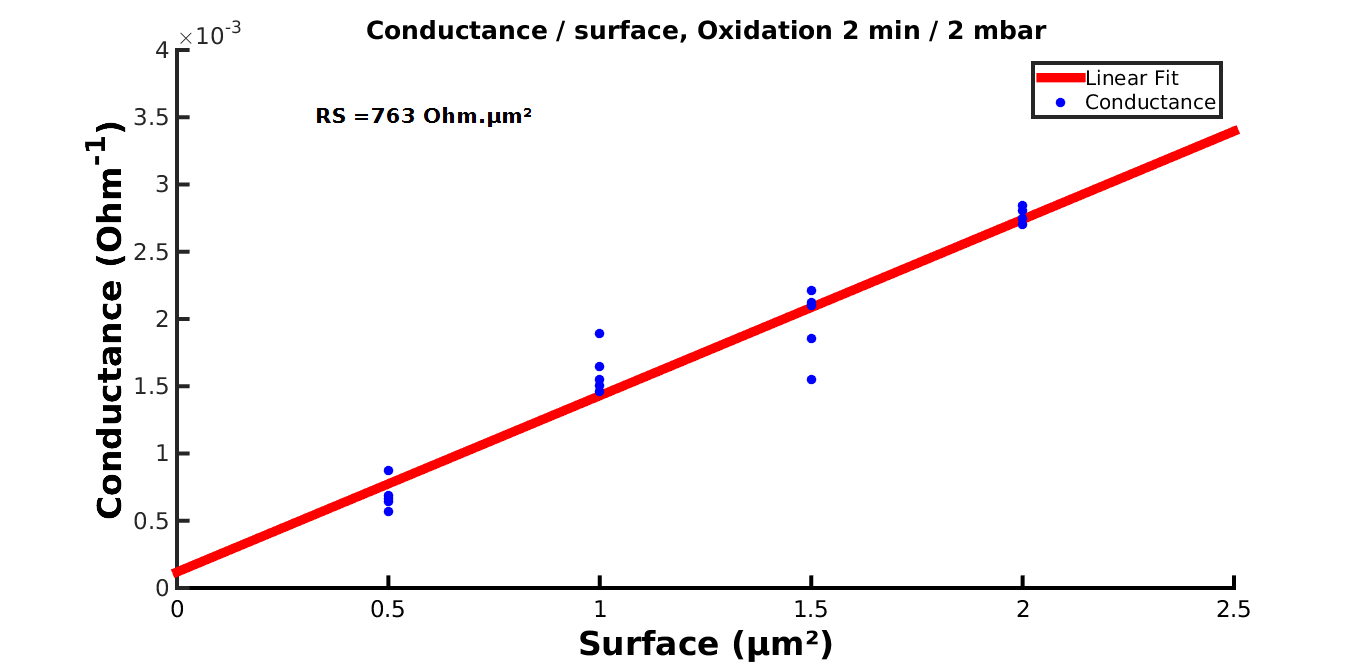
\includegraphics[width=12cm]{ConductanceFitOx.png}
                    \caption{Conductance in function of surface area for a regular oxidized sample}
                    \label{Regularox}
                \end{figure}
                                
                \[RS=7\Omega.\mu m^2\]
                
                RS is ten times less important than for the strong oxidation which means that the layer of oxide is ten times thinner.
                These three references give us a base to evaluate the quantity of oxide left when we will etch it. For example, if we find a resistance around $1k\Omega$, we can assume that the thickness of oxide is close to the thickness of the regular oxidation.
                                
                \subsection{Plasma Etching : Position of the sample}
                
                Then, I wanted to check if the plasma is uniform. We do not know if it affects equally all the areas of the sample stage or not. This is why I've made several tests where I placed 4 samples on the sample stage and did the evaporation. The Figure \ref{PlasmaPosition} shows the results of these tests. We can see that the position does not affect much the resistance of the sample so we can assume that the etching is quite uniform. And another conclusion of this graphe is that 10 min of plasma are enough to etch all the Al oxide : there is no surface dependance like for the oxidized samples and the resistance is about the same order of magnitude than the clean contact junction.
                
                \begin{figure}
                    \centering
                    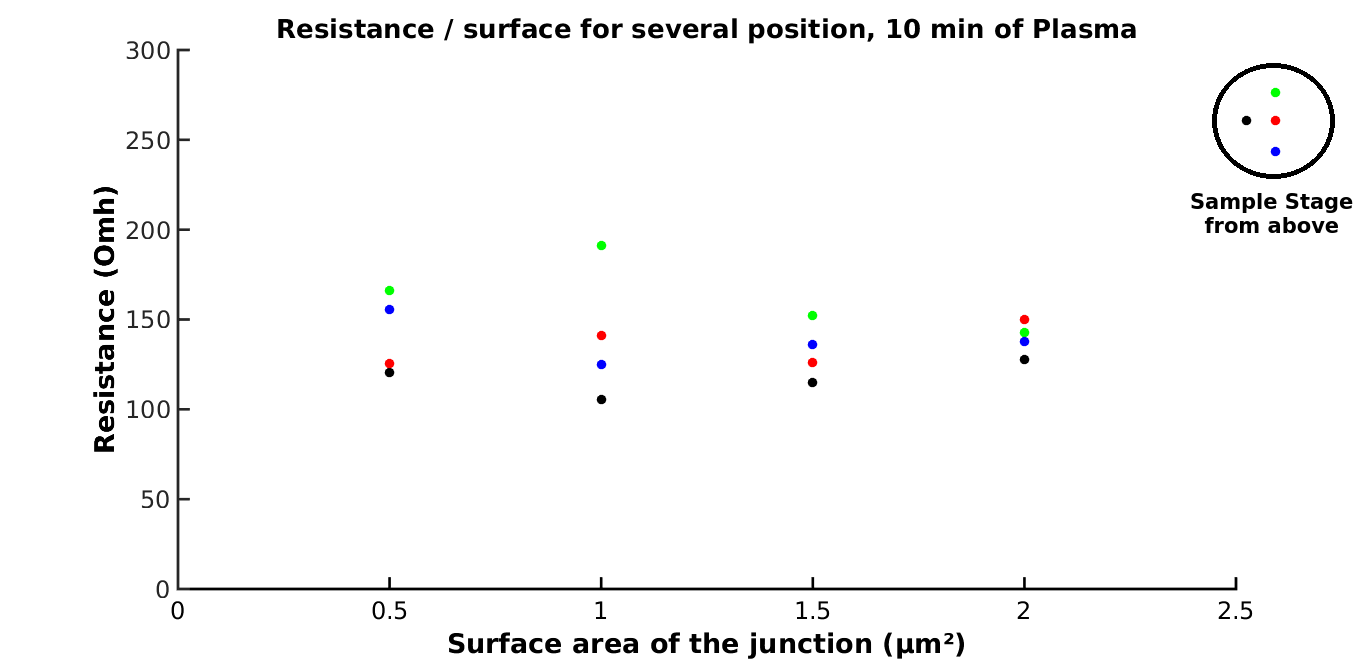
\includegraphics[width=12cm]{R_Position.png}
                    \caption{Resistance in function of surface for different positions of the samples on the LISA's sample stage}
                    \label{PlasmaPosition}
                \end{figure}               
                
                
                \subsection{Time of plasma}
                
                The time during which the sample is exposed to the plasma is important and determine how much oxide will be etched and implicitely the resistance of the sample. I followed the same procedure all along and only changed the etching duration.
                In Figure \ref{SEMPlasma} there are some good samples made with plasma etching. Some samples also turned out to become failures, there are SEM images with explanation in Appendix \ref{badplasma}.
                 
                 
                The Figure \ref{PlasmaTimeBefore} shows the resistance compared to plasma etching duration before the cleaning of the plasma gun. We can see that there is not a lot of differences between 10 and 20 minutes but the more relevant result is what we can see on the Figure \ref{PlasmaTimeAfter}, with samples made after the cleaning, it seems that les than 5 minutes is enough to etch all the oxide, since the results are very similar, yet for totally different duration times. It means that the cleaning had an effect on the plasma settings.
                \begin{figure}
                    \centering
                    \begin{subfigure}[t]{0.48\textwidth}
                    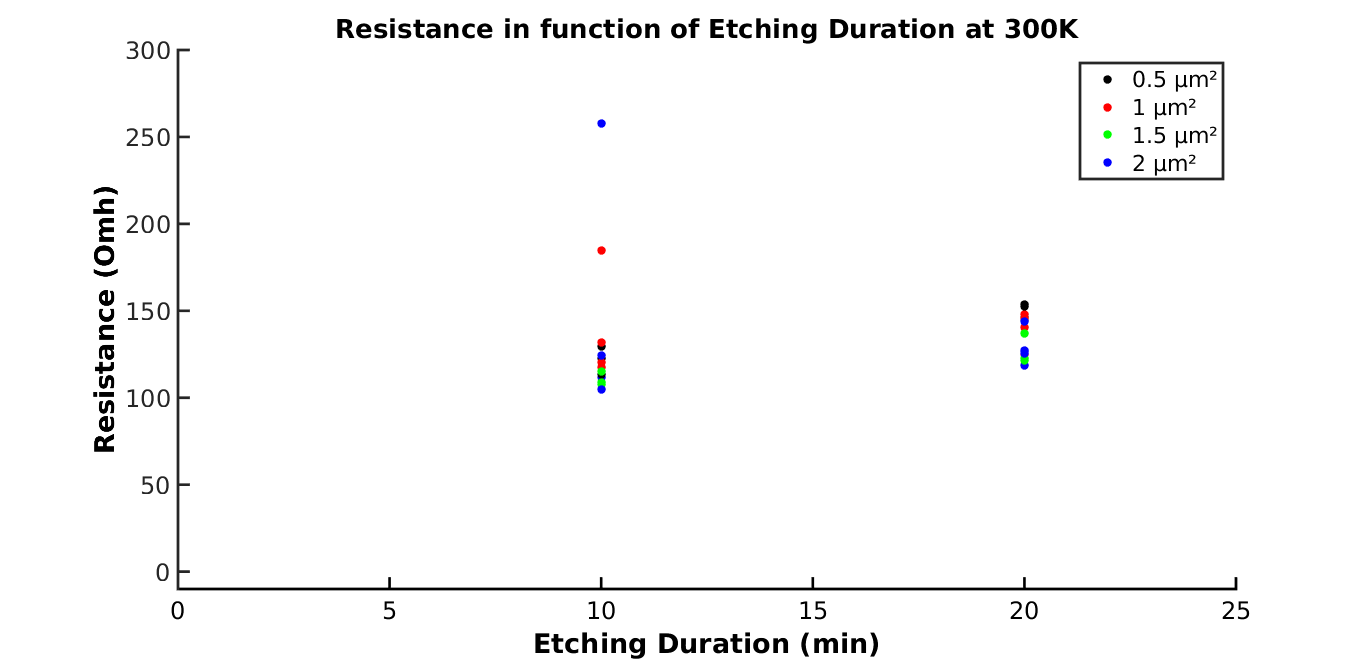
\includegraphics[width=7.2cm]{R_TimeBefore.png}
                    \caption{Resistance in function of Plasma Etching duration before the cleaning}
                    \label{PlasmaTimeBefore}
                    \end{subfigure}
                    \begin{subfigure}[t]{0.48\textwidth}
                    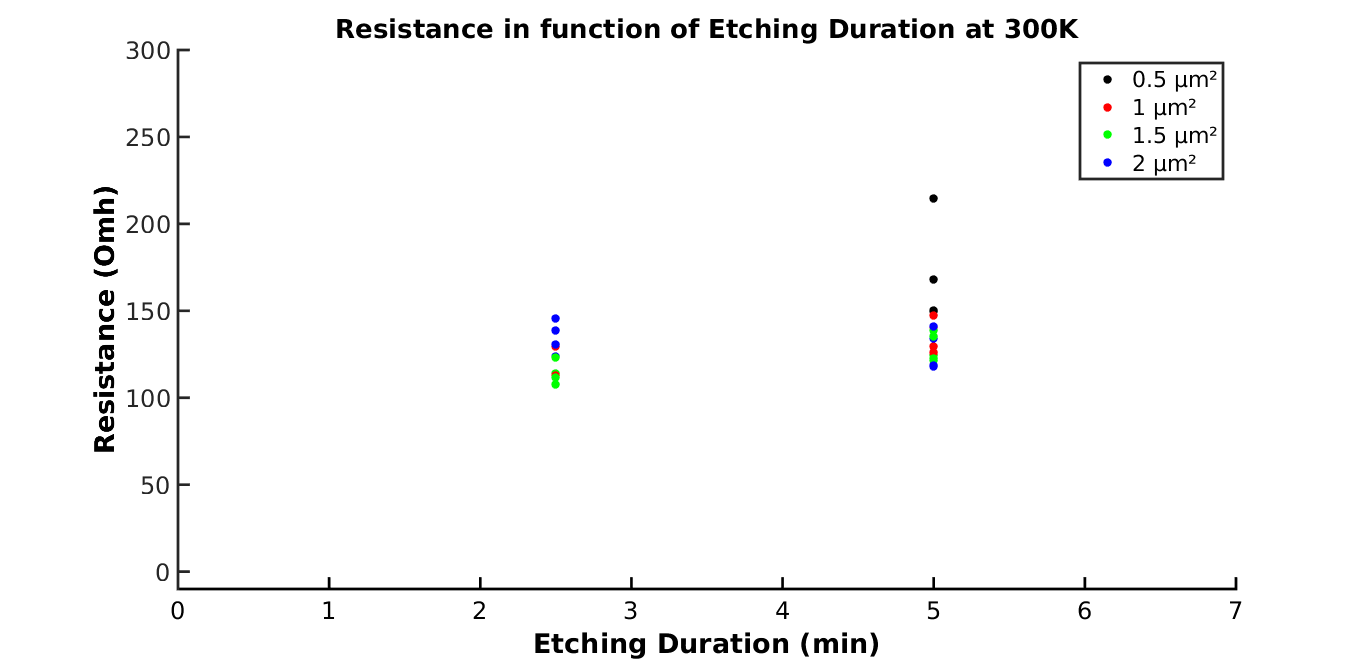
\includegraphics[width=7.5cm]{R_TimeAfter.png}
                    \caption{Resistance in function of Plasma Etching duration after the cleaning}
                    \label{PlasmaTimeAfter}
                    \end{subfigure}
                \end{figure}
                
                \section{Low temperature measurements}
                
                \subsection{NIS Junction}
                
                Thanks to the dilution cryostat I was able to cool down some samples down to 50mK. Of course the pads on the sample stage are in a limited number so that I had to chose the best samples to bound and to cool down. 
                
                
                
                
                \subsection{Plasma etched samples}
                
                
                
                \section{Summary of the results}
                
                
                
